\documentclass{article}
\usepackage{graphicx}
\usepackage{tabularx}
\usepackage{booktabs}

\title{Problem Statement and Goals\\\progname}

\author{\authname}

\date{}

%% Comments
\usepackage{color}
\newif\ifcomments\commentstrue %displays comments
%\newif\ifcomments\commentsfalse %so that comments do not display
\ifcomments
\newcommand{\authornote}[3]{\textcolor{#1}{[#3 ---#2]}}
\newcommand{\todo}[1]{\textcolor{red}{[TODO: #1]}}
\else
\newcommand{\authornote}[3]{}
\newcommand{\todo}[1]{}
\fi
\newcommand{\wss}[1]{\authornote{blue}{SS}{#1}} 
\newcommand{\plt}[1]{\authornote{magenta}{TPLT}{#1}} %For explanation of the template
\newcommand{\an}[1]{\authornote{cyan}{Author}{#1}}
%% Common Parts
\newcommand{\progname}{4TB6 - Mechatronics Capstone} % PUT YOUR PROGRAM NAME HERE
\newcommand{\authname}{Team \#5, Locked \& Loaded
\\ Abi Nevo, nevoa
\\ Elsa Bassi, bassie
\\ Steffi Ralph, ralphs1
\\ Abdul Iqbal, iqbala18
\\ Stephen De Jong, dejons1
\\ Anthony Shenouda, shenoa2} % AUTHOR NAMES                  

\usepackage{hyperref}
    \hypersetup{colorlinks=true, linkcolor=blue, citecolor=blue, filecolor=blue,
                urlcolor=blue, unicode=false}
    \urlstyle{same}


\begin{document}
\maketitle
\begin{figure}[h!]
  \centering
  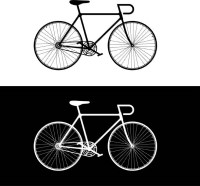
\includegraphics[width=0.4\linewidth]{../BikeLogo.jpg}
\end{figure}

\begin{table}[hp]
\caption{Revision History} \label{TblRevisionHistory}
\begin{tabularx}{\textwidth}{llX}
\toprule
\textbf{Date} & \textbf{Developer(s)} & \textbf{Change}\\
\midrule
Sep 25 & Steffi & Completed\\
\bottomrule
\end{tabularx}
\end{table}

\newpage
\section{Problem Statement}

\subsection{Problem}

There are many problems associated with bike locks today.  People often forget or lose their keys, lock or combination.  Additionally, current locking systems are often not comprehensive – they may not lock all parts of the bike that can be stolen, (the seat, front and back wheels and frame). 

Furthermore, the problem stretches beyond the locking mechanisms; bike locks can be bulky, heavy and dangerous to carry around and it can also be tedious to find and lock one’s bike to an external frame.  The combination of these issues can lead to individuals leaving their bikes without properly locking them.  The city of Toronto reports an average 3625 stolen bikes annually, and the Canadian Cycling Magazine estimates that only 15-20\% of stolen bikes are reported which indicates a rather expansive problem that needs to be solved [1,2]. 

Our team presents the Smart Lock, which is a bike lock that is locked/unlocked through a cellphone application.  Users can secure their bikes automatically, eliminating the need for manual locking through keys and a combination.  The application includes a GPS component to locate the bike in case the user forgets where they parked it or in the event that it is stolen.  Additionally, the Smart Lock is intended to be mounted permanently on the bike frame, eliminating the need to carry a lock.  The sleek design will ensure that the lock is unobtrusive while riding. 


\subsection{Inputs and Outputs}

\begin{table}[hp]
  \begin{center}
    \begin{tabular}{| l | r |}
    \hline
      \textbf{Inputs} & \textbf{Outputs}\\
      \hline
      SignalLock (to lock latch)  & LatchLocked\\
	    SignalUnlock (to unlock) & LatchUnlocked\\
	    SignalOpened & LockOpened\\
	    SignalClosed & LockClosed\\
	    BatteryPower & Battery \% Status\\
	    GpsLocation & BikePosition\\
	    \hline
    \end{tabular}
  \end{center}
\end{table}

\subsection{Stakeholders}

Cyclists or aspiring cyclists interested in improving the efficiency, usability and security of locking their bike.

\subsection{Environment}

Below is a list of the  hardware and software needed to implement the solution to the problem.
Hardware: physical lock, power source, motor/actuator, input device (Bluetooth/ antennae/ transmitter/ receiver), positioning sensors 
Software: phone app

\section{Goals}
\begin{table}[hp]
  \begin{center}
    \begin{tabular}{| p{0.5\linewidth} | p{0.5\linewidth} |}
    \hline
      \textbf{Goals} & \textbf{Measurability}\\
      \hline
      Wireless communication and engagement/disengagement of bike lock  & Quality and distance of signal strength\\
      \hline
      Effective bike lock  & Lock functions, X amount of force before failure\\
      \hline
      Long lasting battery life  & Time - in months \\
      \hline
      Fits on many different styles of bikes & Can easily be mounted to mountain bikes, city bikes, children's bikes and road bikes \\
      \hline
      Easily mount on bike frame & Does not require special tools for mount/dismount\\
      \hline
    \end{tabular}
  \end{center}
\end{table}

\section{Stretch Goals}
\begin{itemize}
\item Integrating with fitness apps (ie. strava) for increased capabilities
\item Integrating the battery with a solar panel for self charging to reduce user interaction with the lock futher
\item GPS location services
\item Cross platform app implementation for accessibility using an Android in addition to an IOS device
\section{References}
\end{itemize}

[1]“bicycle-thefts,” data.torontopolice.on.ca. https://data.torontopolice.on.ca/pages/bicycle-thefts (accessed Sep. 25, 2022).
[2]L. Hansen-Gillis, “Bike thefts are increasing in Canada: Here’s what you can do to protect your bike,” Canadian Cycling Magazine, Nov. 04, 2020. https://cyclingmagazine.ca/sections/news/bike-theft-canada/ (accessed Sep. 25, 2022).
‌
‌

\end{document}